\section{Methods}

Full atom simulations of DNA molecules exist (todo: citations) but are computationally very heavy. In 2007, the group of De Pablo \cite{knotts2007coarse} applied the technique of coarse graining to a molecular simulation of DNA: instead of simulating all atoms, a DNA monomer is represented by three sites: the sugar, the phosphate and the base. For simulations where one is mainly interested in the timescale behaviour or global dynamics of the DNA molecule this is a very good approximation: it is computationally cheap (and easy to optimize) while describing the DNA helical structure quite good. 

\subsection{DNA structure}

In this paper, we follow the approach of Knotts, De Pablo \etal \cite{knotts2007coarse} to model the structure of B-DNA. In Figure \ref{dna_forms}, the main three structural forms of DNA are illustrated.

\begin{figure}[htbp]
\begin{center}
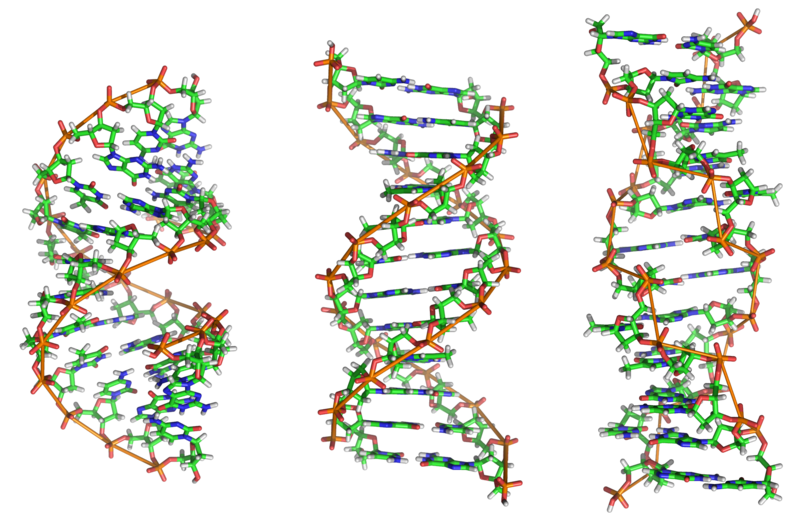
\includegraphics[width=14cm]{dna_forms.png}
\caption{Structural forms of DNA: A-DNA (left), B-DNA (center) and Z-DNA (right). Figure from \href{http://www.molecularstation.com}{molecularstation.com}.}
\label{dna_forms}
\end{center}
\end{figure}


The algorithm to build up a single strand is to follow the screw symmetry of B-DNA by placing consecutive monomers on the $z$-axis of space (separated by an axial rise of $3.38$\,\Angstrom), and rotating each consecutive monomer by an angle of $36$ degrees. In practice, this means that if a monomer is placed at location $(r, \phi, z)$, the consecutive monomer on the same strand is placed at $(r, \phi + 36\degree, z + 3.38\,\text{\Angstrom})$. To build up the complementary strand (yielding the characteristic double stranded helical structure of DNA), an atom at $(x, y, z)$ on the first strands has its complementary atom on the other strand at $(x, -y, -z)$ with the $x$-axis taken orthogonal to the helical axis and always along the line connecting the complementary bases of the complementary monomers (i.e. the $x$-axis also rotates $36\degree$ along the $z$-axis for consecutive base pairs along the double strand).

Knotts \etal \cite{knotts2007coarse} used the DNA molecular data of ref. \cite{crcBiochem1976}, and averaged positions for each of the three sites per nucleus yielding the data in table \ref{dnaStructureData}.

\begin{table}[htdp]
\caption{Structural data for B-DNA helices, calculated by Knotts \etal \cite{knotts2007coarse}.}
\begin{center} \footnotesize
\begin{tabular}{|l|rrrrc|c|}
\hline
 &\ \  x (\Angstrom)\ \ &\ \  y (\Angstrom)\ \  &\ \  z (\Angstrom)\ \  &\ \  r (\Angstrom)\ \  &\ \  $\phi$ (degrees)\ \  & \ \ Mass (amu) \\
\hline
Phosphate (P) & -0.628 & 8.896 & 2.186 & 8.918 & 94.038 & 94.97 \\
Sugar (S) & 2.365 & 6.568 & 1.280 & 6.981 & 70.197 & 83.11 \\
Adenine base (Ab) & 0.575 & 0.516 & 0.051 & 0.773 & 41.905 & 134.1\\
Thymine base (Tb) & 0.159 & 2.344 & 0.191 & 2.349 & 86.119 & 125.1\\
Cytosine base (Cb) & 0.199 & 2.287 & 0.187 & 2.296 & 85.027 & 110.1\\
Guanine base (Gb) & 0.628 & 0.540 & 0.053 & 0.828 & 40.691 & 150.1\\
\hline
\end{tabular}
\end{center}
\label{dnaStructureData}
\end{table}%

Schematically, this structure yields the major and minor grooves as illustrated in Figure \ref{schematic_knotts}. The phosphate and sugar sites on the backbone of the molecule are placed at the centers of mass of the molecules; bases Ab and Gb are placed at the N1 position of the B-DNA isoform; bases Tb and Cb at the N3 position. 

\begin{figure}[h]
\begin{center}
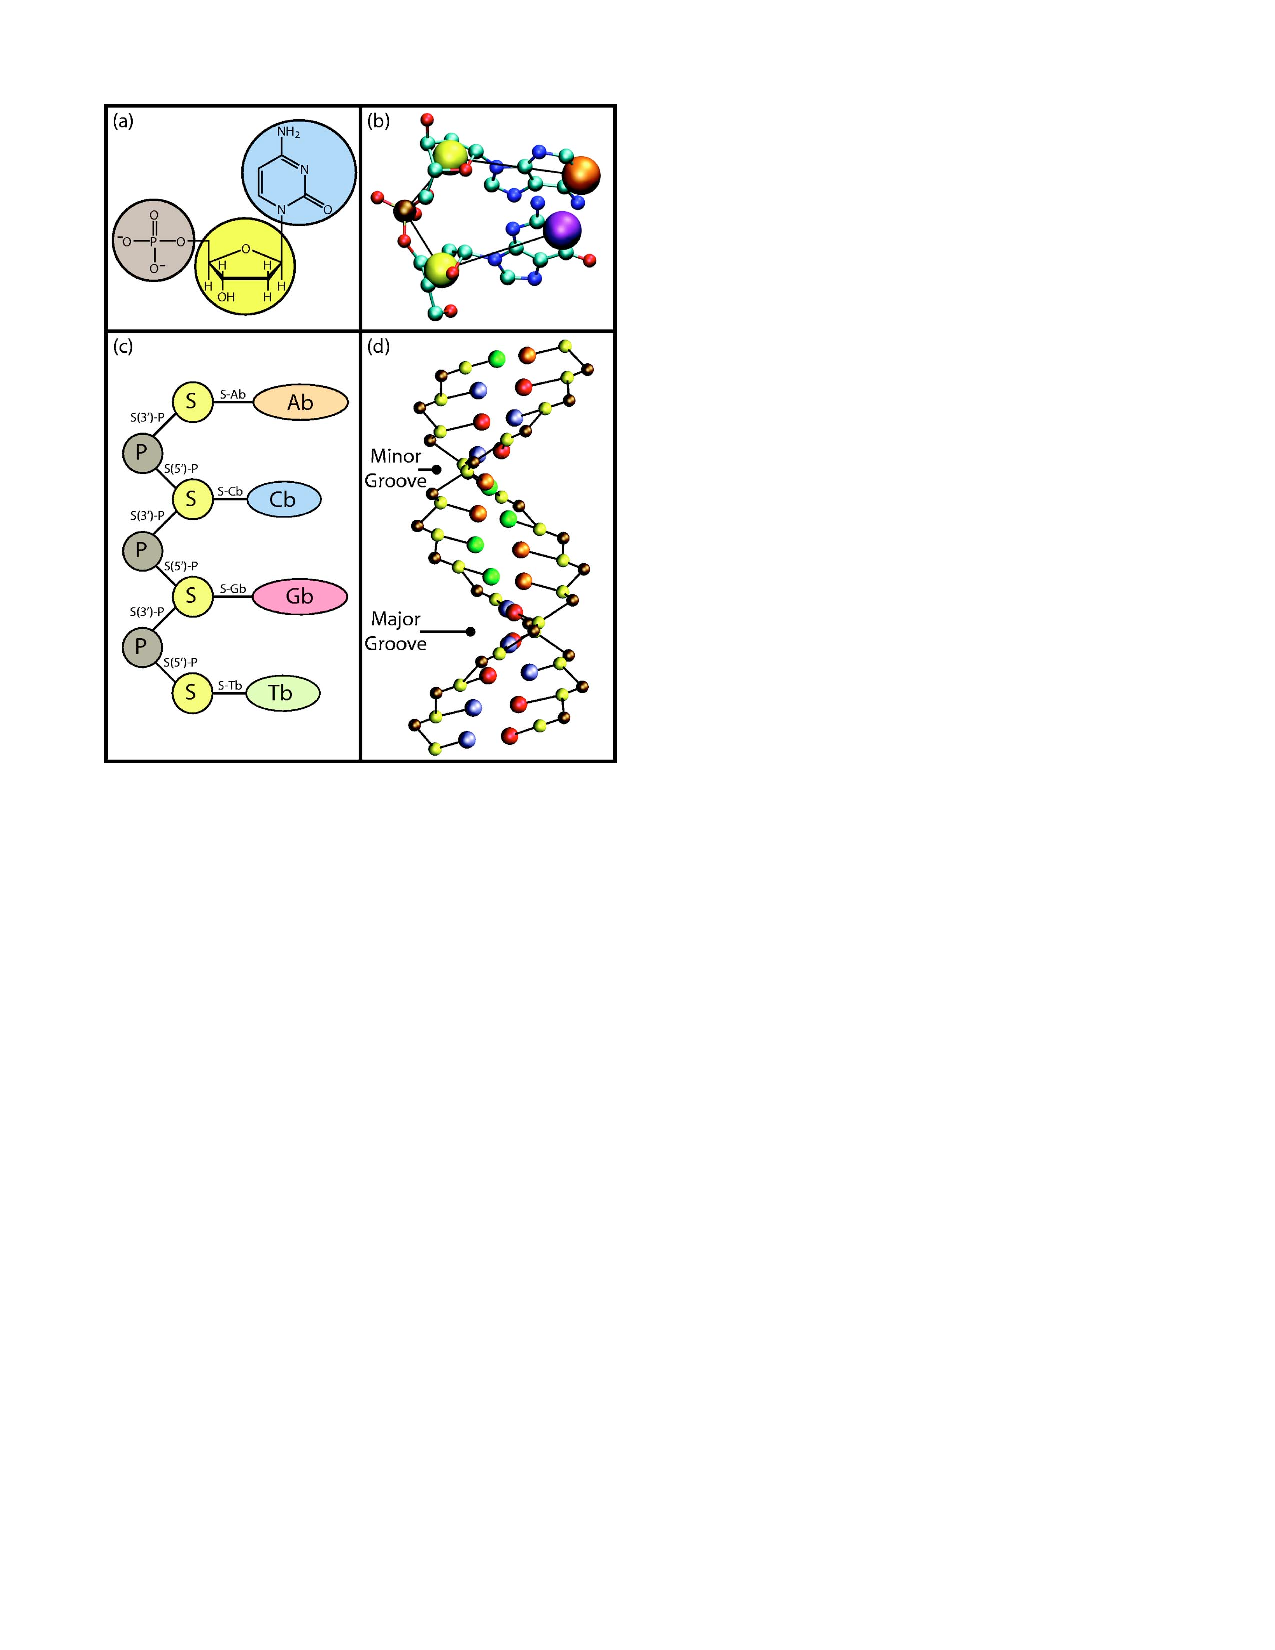
\includegraphics{schematic_structure_knotts}
\caption{The schematic structure of the model for B-DNA, from Knotts \etal \cite{knotts2007coarse}. Note the placing of the three sites per nucleus relative to the original atomic structure in the upper right panel.}
\label{schematic_knotts}
\end{center}
\end{figure}




\subsection{Interactions}

The potential energy of the complete system consists of
\begin{equation}
V_\text{total} = V_\text{bond} + V_\text{angle} + V_\text{dihedral} + V_\text{stack} + V_\text{bp} + V_\text{ex} + V_\text{qq}.
\end{equation}
The strengths of the individual iteractions will be expressed in terms of the energy unit $\varepsilon$, taken to be $0.26$\,kcal/mol. The potential energies are taken mainly from the potential terms as defined by Florescu \& Joyeux \cite{florescu2011thermal}, and are an improvement over the original terms by Knotts \etal \cite{knotts2007coarse}. However, in the end they are very much alike and interchangeable; and we opt for the conventions of the Florescu paper primarily because they are more clearly formulated. We will now sketch the specific potential energy terms one by one, but first we define a few constants regularly used in the potentials.

\begin{table}[hbt]\begin{center}
\begin{tabular}{llll}
Parameter & Value \qquad \qquad \qquad \qquad & Parameter & Value\\
\hline
$\varepsilon$ & $1.81\times10^{-21}$ Joule/particle\qquad\qquad & $k_\phi$ & $4\varepsilon$ \\
$k_1$ & $10^{20}\varepsilon$ in Joule/(\AA)$^2$ & $\varepsilon_\text{GC}$ & $16\varepsilon$\\

$k_2$ & $100\times10^{20}\varepsilon$ in Joule/(\AA)$^2$ & $\varepsilon_\text{AT}$ & $4\frac{2}{3} \varepsilon_\text{GC}$ \\
$k_\theta$ & $400\varepsilon$ per radian$^2$ & & \\
\end{tabular}
\caption{Regularly used energy constants for the potential energies, used by Knotts \etal \cite{knotts2007coarse}.}\end{center}
\end{table}

\paragraph{Bond potential} The typical expression for the intramolecular bonds between molecules in the same DNA strand is a sum over all bonds of a quadratic and a quartic potential term
\begin{equation}
V_{\text{bond}} = \sum_i^{N_{\text{bond}}} \left[ k_1 \left(d_i - d_{0_i}\right)^2 + k_2 \left(d_i - d_{0_i}\right)^4\right]
\end{equation}
(the `stretch' term) around equilibrium distances $d_{0_i}$ as defined in the standard B-form structure of double strand DNA, and coupling constants $k_1$ and $k_2$.

\paragraph{Bond angle potential} The angle that forms between three consecutively bound sites in a DNA strand is regulated by the sum over all bond angles of the quadratic term (`bend' force)
\begin{equation}
V_\text{angle} =  \sum_i^{N_\text{angle}} \frac{k_\theta}{2} \left( \theta_i - \theta_{0_i} \right)^2
\end{equation}
where we define an equilibrium angle $\theta_0$ from the DNA B-form, and a constant $K_\theta = 400\varepsilon / (\text{radian})^ 2$.

\paragraph{Dihedral angle potential} The third and last potential defining the structural properties of the strand regulates the dihedral angle between four consecutive bound sites on the same strand
\begin{equation}
V_\text{dihedral} =  \sum_i^{N_\text{dihedral}} k_\phi \left[ 1 - \cos (\phi_i - \phi_{0_i}) \right]
\end{equation}
with $\phi_{0_i}$ the equilibrium dihedral angle from the DNA B-form definitions, and constant $k_\phi = 4\varepsilon$.

\paragraph{Stacking potential} The stacking potential is a Leonard-Jones type potential describing the base stacking phenomena and regulates the rigidity of the DNA backbone,
\begin{equation}
V_\text{stack} =  \sum_{i<j}^{N_\text{stack}} \varepsilon \left[ \left(\frac{r^0_{ij}}{r_{ij}} \right)^{12} - 2\left(\frac{r^0_{ij}}{r_{ij}} \right)^{6} + 1\right]
\end{equation}
modeled with an effective cut-off distance of $9$\,\Angstrom because of over which . It is important to observe that this induces not only a stacking interaction between the $i$th and $(i+1)$th base, but also between the $i$th and $(i+2)$th base. (Hence the sum over all stackings $i$ and $j$, with $i < j$ to avoid double counting). $\sigma_{ij}$ depends on the type of bases for which the stacking is calculated.

\paragraph{Basepairing potential} A hydrogen bonding interaction between two complimentary bases (zero if not complementary) is written as
\begin{equation}
V_\text{bp} =  \sum_{\text{base pairs}}^{N_\text{bp}} \varepsilon_{\text{bp}_i} \left[ 5\left(\frac{r^0_{\text{bp}_i}}{r_{ij}} \right)^{12} - 6\left(\frac{r^0_{\text{bp}_i}}{r_{ij}} \right)^{10} + 1\right]
\end{equation}
where we have $r^0_{bp}$ depending on the type of complimentary basepair and coupling constants $\varepsilon_\text{GC}$ and $\varepsilon_\text{AT}$.

\paragraph{Exclusion potential} In the original and follow-up versions of the 3SPN model (Knotts \etal \cite{knotts2007coarse}, Sambriski \etal \cite{sambriski2009mesoscale}) a Leonard-Jones type potential was used to describe excluded volume interactions between mismatched bases (yielding $\sigma_0 = 1.0 \times 2^{-1/6}$\,\Angstrom) and other molecules (even on other strands) that do not interact via the Coulomb or basepairing potential (yielding $r_0 = 6.86 \times 2^{-1/6}$\,\Angstrom):
\begin{equation}
V_\text{excl} =  \sum_{i<j}^{N_\text{ex}}\begin{cases} 4\varepsilon \left[ \left(\frac{r_{0}}{r_{ij}} \right)^{12} - \left(\frac{r_{0}}{r_{ij}} \right)^{6} \right] + \varepsilon \qquad &\text{if }r_{ij} < d_\text{cut}, \\ 0 \qquad &\text{if }r_{ij} \geq d_\text{cut} \end{cases} \end{equation}
where a cut-off value of $d_\text{cut} = 5.86$\,\Angstrom\ is imposed. This will make sure two strands do not cross each other when simulating DNA hybridisation, and also that a single strand does not cross itself during a hairpin formation simulation. Florescu \& Joyeux \cite{florescu2011thermal} report that the exclusion potential is not necessary when simulating long double stranded DNA helices; we decided however to keep this potential for the above reasons. The cut-off value of $5.86$ \Angstrom\ we use, however, is a little bit smaller than the original value in Knotts and Sambriski \cite{knotts2007coarse, sambriski2009mesoscale} where $6.86$ \Angstrom\ is used; we find that by decreasing the cut-off value slightly we massively improve the (local) stability of the system without losing the crucial advantages of the exclusion potential.

\paragraph{Coulombic potential} The final potential in our model is the screened electrostatic Coulomb interaction between the phosphate molecules situated on the backbone of the DNA strands. It is modeled using a Debye-H\"uckel approximation with a Debye length $\kappa_D$ depending on the salt concentration of the environment,
\begin{equation}
V_\text{qq} =\sum_{i<j}^N  \frac{q_i q_j}{4\pi \varepsilon_0 \varepsilon_k r_{ij}} \exp \left(- \frac{r_{ij}}{k_D}  \right)
\label{coulomb}\end{equation}
where the Debye length can be written as
\begin{equation}
\kappa_D = \left( \frac{\varepsilon_0 \varepsilon_k RT}{2N^2_A e^2 I} \right)^{0.5}
\end{equation}
where we use the vacuum permittivity $\varepsilon_0$, Avogadro´s number $N_A$, the electronic charge $e$ and the ionic strength $I$. For the default value of the ionic strength [Na$^+$]=50 mM (milimolair, equal to milimol/liter) this yields $\kappa_D$ = 13.603\,\Angstrom. The other values in \ref{coulomb} are the dielectric constant $\varepsilon_k = 78$ for water, and the charges on the interacting molecules (phosphates, with $q_i = -1$ so $q_i q_j = 1$).

The interactions are defined so that two molecules are excluded from the nonbonded interactions if they constitute a bond. On top of that, $V_\text{stack}$, $V_\text{bp}$ and $V_\text{ex}$ are modeled as mutually exclusive. Our codebase makes sure that this is handled correctly, to avoid the unphysical pairing of bases on the same strand or to avoid cases where an exclusion potential is working on two sites already interacting via Coulombic interaction. All non-specified geometric and interaction constants are taken from Table III in \cite{knotts2007coarse}, which we reproduce in Table \ref{geometricConstants} for consistency's sake.

\begin{table}[htb]
\begin{tabular}{lccc}
\hline
Bond&$d_0$ (\AA)&Bond Angle& $\theta_0$ (degree) \\
\hline
S(5')-P & 3.899 & S(5')-P-(3')S & 94.49\\
S(3')-P & 3.559 & P-(5')S(3')-P & 120.15 \\
S-Ab & 6.430 & P-(5')S-Ab & 113.13\\
S-Tb & 4.880 & P-(3')S-Ab & 108.38\\
S-Cb & 4.921 & P-(5')S-Tb & 102.79\\
S-Gb & 6.392 & P-(3')S-Tb & 112.72\\
&&P-(5')S-Cb & 103.49\\
&& P-(3')S-Cb & 112.39\\
&& P-(5')S-Gb & 113.52\\
&& P-(3')S-Gb & 108.12\\
& & & \\
\hline
Dihedral Angle & $\phi_0$ (degree) & Nonbonded & Length (\AA) \\
\hline
P-(5')S(3')-P-(5')S & -154.80 & $r^0_{ij}$ & Interaction specific \\
S(3')-P-(5')S(3')-P & -179.17 & $r^0_{\text{bp}_\text{AT}}$ & 2.9002 \\
Ab-S(3')-P-(5')S & -22.60 & $r^0_{\text{bp}_\text{GC}}$ & 2.8694 \\
S(3')-P-(5')S-Ab & 50.69 & $r_0$ (mismatched bases) & $2^{-1/6} (1.0)$ \\
Tb-S(3')-P-(5')S & -33.42 & $r_0$ (otherwise) & $2^{-1/6} d_\text{cut}$ \\
S(3')-P-(5')S-Tb & 54.69 & & \\
Cb-S(3')-P-(5')S & -32.72 & $d_\text{cut}$ & $r^0 \approx 5.86$ \\
S(3')-P-(5')S-Cb	& 54.50 & & \\
Gb-S(3')-P-(5')S & -22.30 & & \\
S(3')-P-(5')S-Gb & 50.66 & & \\
\hline
\end{tabular}\label{geometricConstants}

\caption{Geometric constants for the potential energy functions as defined above. Important to note is that a sugar can bind to a phosphate in a 5' or a 3' sense; S(5')-P represents a sugar-phosphate bond inside the same nucleotide but S(3')-P is a bond between neighboring nucleotides. Bond angles like P-(5')S(3')-P include both kinds of bondings. The table is reproduced from Knotts \etal \cite{knotts2007coarse}.}
\end{table}

Because we work with a space partitioning scheme, we will also truncate the potential energies that we use at a certain chosen truncation length (default at $20$\,\Angstrom) and shift them so that they yield a potential energy of zero when calculated at the truncation distance.

\subsection{Space Partitioning}



\subsection{Dynamics}
